\begin{figure}
    \begin{center}
    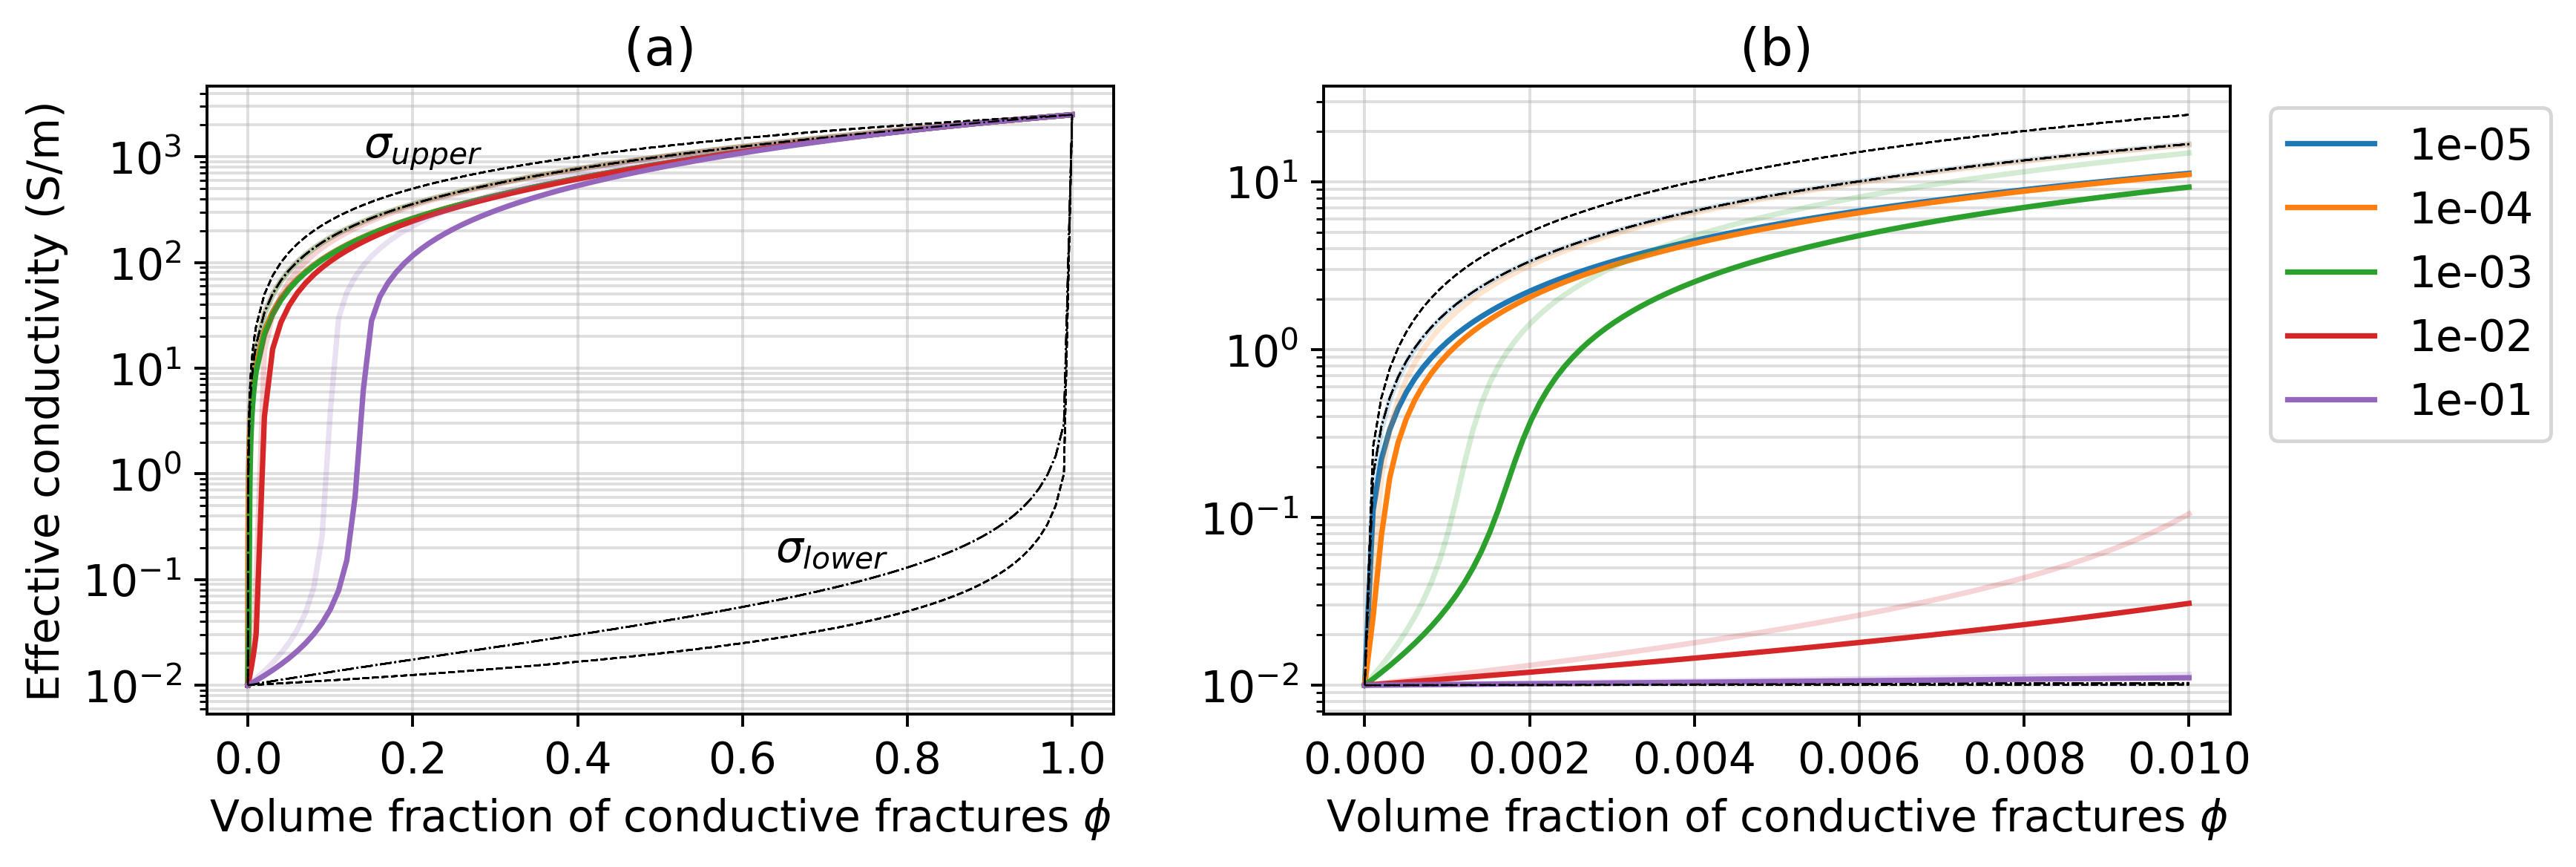
\includegraphics[width=\columnwidth]{figures/phys_prop_model/random_fractures.png}
    \end{center}
\caption{
    Effective, isotropic conductivity for a fractured rock with randomly oriented spheroidal
    cracks for five different aspect ratios, indicated by the legend. The black dashed lines show the upper and lower
    Wiener Bounds, which are identical the volume-weighted arithemtic and harmonic averages of the
    conductivity of the rock (0.1 S/m) and proppant-fluid mixture (2500 S/m).The black dash-dot lines
    are the isotropic Hashin-Shtrikman upper and lower bounds.
    The semi-transparent dotted lines show $\sigma_{x, z}$ from Figure \ref{fig:aligned_fractures}
    Panel (a) shows the
    full range $0 \leq \phi \leq 1$, and panel (b) zooms in to $0 \leq \phi \leq 0.01$.
}
\label{fig:random_fractures}
\end{figure}
